\newif\ifshowsolutions
\showsolutionstrue
\documentclass{article}
\usepackage{listings}
\usepackage{amsmath}
%\usepackage{subfigure}
\usepackage{subfig}
\usepackage{amsthm}
\usepackage{amsmath}
\usepackage{amssymb}
\usepackage{graphicx}
\usepackage{mdwlist}
\usepackage[colorlinks=true]{hyperref}
\usepackage{geometry}
\usepackage{titlesec}
\geometry{margin=1in}
\geometry{headheight=2in}
\geometry{top=2in}
\usepackage{palatino}
\usepackage{mathrsfs}
\usepackage{fancyhdr}
\usepackage{paralist}
\usepackage{todonotes}
\setlength{\marginparwidth}{2.15cm}
\usepackage{tikz}
\usetikzlibrary{positioning,shapes,backgrounds}
\usepackage{float} % Place figures where you ACTUALLY want it
\usepackage{comment} % a hack to toggle sections
\usepackage{ifthen}
\usepackage{mdframed}
\usepackage{verbatim}
\usepackage[strings]{underscore}
\usepackage{listings}
\usepackage{bbm}
\rhead{}
\lhead{}

\renewcommand{\baselinestretch}{1.15}

% Shortcuts for commonly used operators
\newcommand{\E}{\mathbb{E}}
\newcommand{\Var}{\operatorname{Var}}
\newcommand{\Cov}{\operatorname{Cov}}
\newcommand{\Bias}{\operatorname{Bias}}
\DeclareMathOperator{\argmin}{arg\,min}
\DeclareMathOperator{\argmax}{arg\,max}

% do not number subsection and below
\setcounter{secnumdepth}{1}

% custom format subsection
\titleformat*{\subsection}{\large\bfseries}

% set up the \question shortcut
\newcounter{question}[section]
\newenvironment{question}[1][]
  {\refstepcounter{question}\par\addvspace{1em}\textbf{Question~\Alph{question}\!
    \ifthenelse{\equal{#1}{}}{}{ [#1 points]}: }}
    {\par\vspace{\baselineskip}}

\newcounter{subquestion}[question]
\newenvironment{subquestion}[1][]
  {\refstepcounter{subquestion}\par\medskip\textbf{\roman{subquestion}.\!
    \ifthenelse{\equal{#1}{}}{}{ [#1 points]:}} }
  {\par\addvspace{\baselineskip}}

\titlespacing\section{0pt}{12pt plus 2pt minus 2pt}{0pt plus 2pt minus 2pt}
\titlespacing\subsection{0pt}{12pt plus 4pt minus 2pt}{0pt plus 2pt minus 2pt}
\titlespacing\subsubsection{0pt}{12pt plus 4pt minus 2pt}{0pt plus 2pt minus 2pt}


\newenvironment{hint}[1][]
  {\begin{em}\textbf{Hint: }}{\end{em}}

\ifshowsolutions
  \newenvironment{solution}[1][]
    {\par\medskip \begin{mdframed}\textbf{Solution~\Alph{question}#1:} \begin{em}}
    {\end{em}\medskip\end{mdframed}\medskip}
  \newenvironment{subsolution}[1][]
    {\par\medskip \begin{mdframed}\textbf{Solution~\Alph{question}#1.\roman{subquestion}:} \begin{em}}
    {\end{em}\medskip\end{mdframed}\medskip}
\else
  \excludecomment{solution}
  \excludecomment{subsolution}
\fi



%%%%%%%%%%%%%%%%%%%%%%%%%%%%%%
% HEADER
%%%%%%%%%%%%%%%%%%%%%%%%%%%%%%

\chead{
  {\vbox{
      \vspace{2mm}
      \large
      Machine Learning \& Data Mining \hfill
      Caltech CS/CNS/EE 155 \hfill \\[1pt]
      Miniproject 1\hfill
      February 2019. \\
    }
  }
}

\begin{document}
\pagestyle{fancy}



%%%%%%%%%%%%%%%%%%%%%%%%%%%%%%
% PROBLEM 1
%%%%%%%%%%%%%%%%%%%%%%%%%%%%%%

\newpage

\section{Introduction [10 points]}

\medskip
\noindent\textbf{Group members: } Frank Kou, James Wei \\
\noindent\textbf{Group name: } 343 \\
\noindent\textbf{Division of labor: } James did basic visualization. Frank implemented first and second method of matrix factorization as well as their corresponding visualizations. James did third method of matrix factorization as well as its correspoding visualization. James and Frank both thought of ideas for 'interesting' visualizations for blog post. James wrote blog post. Frank and James wrote their corresponding sections for report.
\newpage


\section{Basic Visualizations [20 points]}
\medskip
\noindent\textbf{Plots}\\
\begin{center}
	
\includegraphics[width=12cm]{Pictures/Basic_all}
	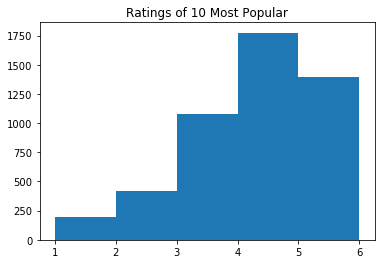
\includegraphics[width=12cm]{Pictures/Basic_popular}
	
\includegraphics[width=12cm]{Pictures/Basic_highest}
	
\includegraphics[width=12cm]{Pictures/Basic_action}
	
\includegraphics[width=12cm]{Pictures/Basic_adventure}
	
\includegraphics[width=12cm]{Pictures/Basic_animation}
\end{center}
\newpage
\noindent\textbf{Analysis}\\
In general, we see that across most of the charts (except "Ratings of 10 Highest Rated"), 4 was the highest frequency rating. The general trend for number of ratings is that 4 got the highest, followed by 3, then 5, 2, 1. The one exception is the 10 most popular movies which has number of ratings as 4, 5, 3, 2, 1. This maybe attributed to a bias that the movie is popular and thus it must be good, which explains why in this case, there are more 5 ratings than 3 ratings. Another trend we noticed was that the graphs are mostly left skewed. They all have very similar shapes. For the most part, the results are what we expected to see. We expected the average and mode to be either 3 or 4 because we believe that people generally give more optimistic ratings. Their scales are set higher. That is, an average movie would get somewhere between a 3 and 4, instead of being a 3. The shapes are also what we expected to see because we felt that people generally dislike giving 1 or 2 ratings. Afterall, it is a movie, which is entertainment. The movie must be extremely horrible or the critic must be very harsh for 1 ratings to be given. However, we did not expect that the ratings of the 10 highest rated movies to be all 5. We thought there would be a majority of 4 and 5 ratings but not all 5. Upon closer inspection, we saw that with most of these movies, they were only rated by either 1 or 2 people. Therefore, if a movie only got a single rating and it was a 5, then it would have a 5 rating overall and thus have the highest average rating possible. Seeing this circumstance makes sense. We see that the ratings of the most popular movies are different from the ratings of the 10 best movies. First of all, the sample size of the best movies are too small. They are outliers, movies that only got 1 or 2 ratings. We see that the most popular movies follow the rating trend of all the rest of the graphs while  the ratings for the best movies were all 5. We see that the ratings for the three genres we chose, action, adventure, and animation, were all very similar. They had similar plot shapes as each other as well as the plot of all the ratings. 
\newpage

\section{Matrix Factorization Methods [40 points]}
\medskip
\noindent\textbf{Normal SVD Plots }\\
\begin{center}
	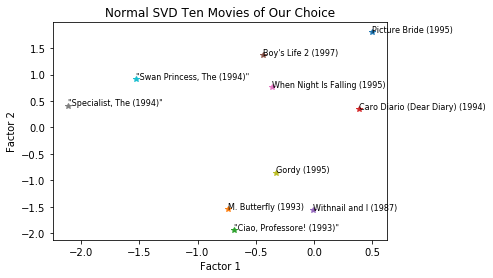
\includegraphics[width=16cm]{Pictures/Normal_choice}
	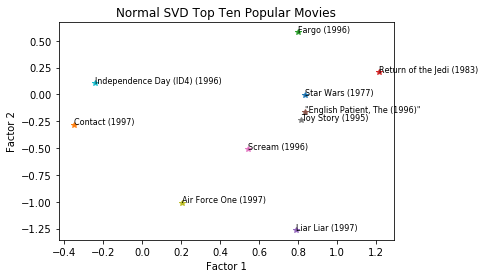
\includegraphics[width=16cm]{Pictures/Normal_popular}
	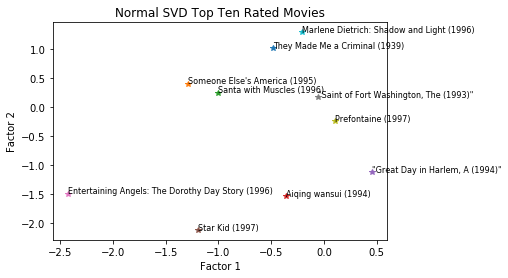
\includegraphics[width=16cm]{Pictures/Normal_highest}
	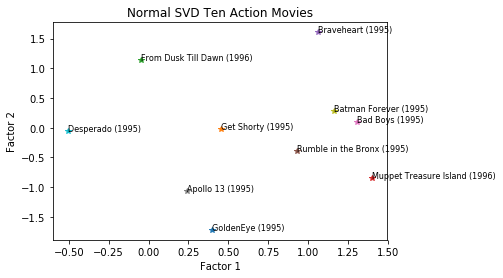
\includegraphics[width=16cm]{Pictures/Normal_action}
	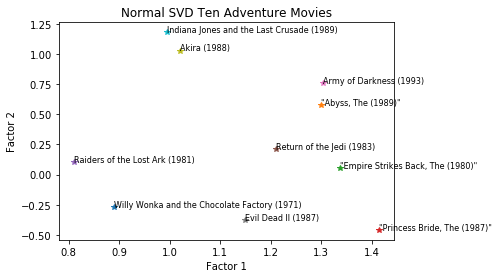
\includegraphics[width=16cm]{Pictures/Normal_adventure}
	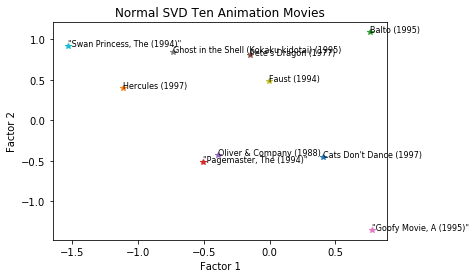
\includegraphics[width=16cm]{Pictures/Normal_animation}
	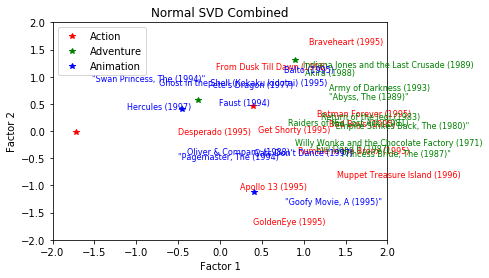
\includegraphics[width=16cm]{Pictures/Normal_combined}
\end{center}
\newpage
\noindent\textbf{SVD with Bias Plots }\\
\begin{center}
	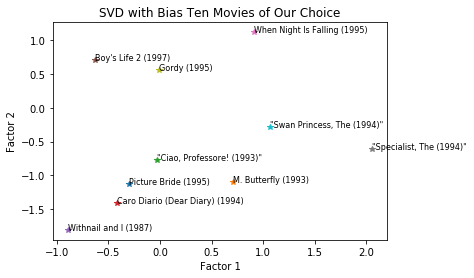
\includegraphics[width=16cm]{Pictures/Bias_choice}
	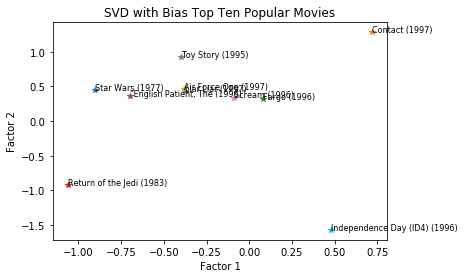
\includegraphics[width=16cm]{Pictures/Bias_popular}
	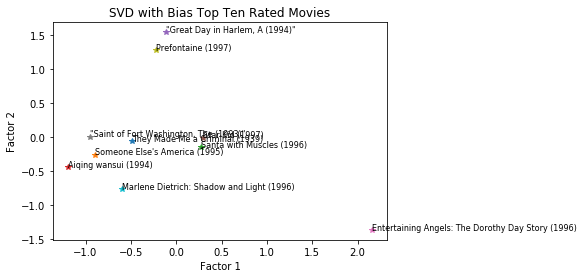
\includegraphics[width=19cm]{Pictures/Bias_highest}
	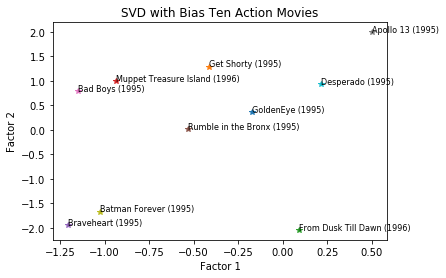
\includegraphics[width=16cm]{Pictures/Bias_action}
	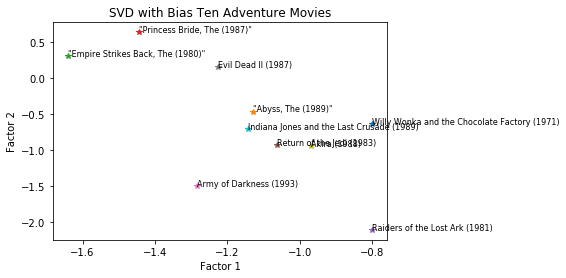
\includegraphics[width=19cm]{Pictures/Bias_adventure}
	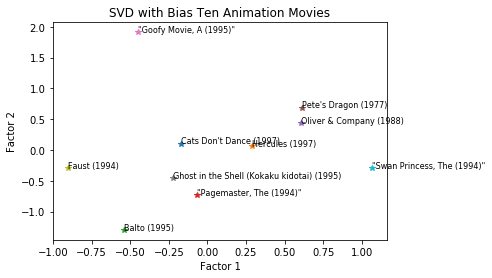
\includegraphics[width=16cm]{Pictures/Bias_animation}
	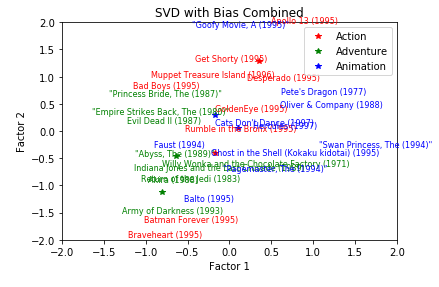
\includegraphics[width=16cm]{Pictures/Bias_combined}
\end{center}
\newpage
\noindent\textbf{Off-the-shelf Implementation Plots }\\








\noindent************************************************************************************\\
TODO post your visualiztions\\ 
************************************************************************************\\
\begin{center}
\end{center}
\newpage









\noindent\textbf{Description }\\
Normal SVD - This is the SVD that we used from Homework 5. This is a matrix decomposition method used for reducing a matrix to its constituent parts in order to predict a full matrix that is missing many values. In our case, we have a M x N user by movie matrix (943 users x 1682 movies). We split this into latent factors matrix $U^T$ and V with size M x k and k x N respectively, where k = 20. \\
SVD with bias - This is like the normal SVD but we incorporate bias. \\
Off-the-shelf - ************ TODO ***************\\
\\

\noindent\textbf{Methods }\\
Normal SVD works by splitting an M x N matrix and tries to learn a latent factor model U and V. $U^T$ and V have size M x k and k x N respectively. This is done by using gradient decent and stopping when we have met our stopping condition. We use Frobenius Norm. When we have successfuly found our U and V, we can multiply the matrices together to get the full matrix and predict what rating each user gives to each movie. In our project, we were given that k has to equal 20. To find the other parameters, we created test cases and plots to determine our parameters. We found out that using an regulizer constant of 0.1 and epsilon of 0.0001 minimized our test error. See below. 
\begin{center}
	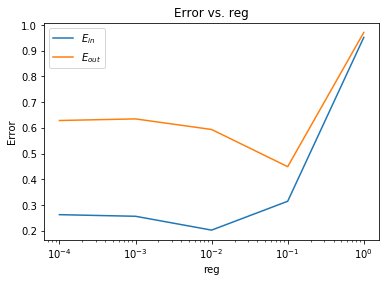
\includegraphics[width=8cm]{Pictures/1_reg}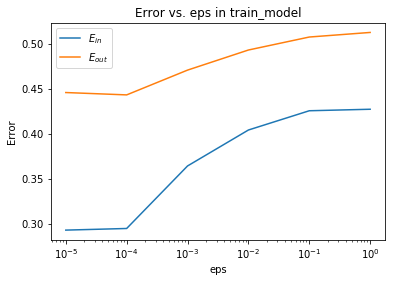
\includegraphics[width=8cm]{Pictures/1_eps}
\end{center}
SVD bias works the same way as normal SVD, except this time we incorporate a bias that we find using gradient decent. This is so we can model the global tendency of a movie's average rating and model the tendency of how a user rates on average. This keeps U and V more focused on variability between users and movies. This is especially important because different users, for example, have different opinions on how ratings are given. One user may be very optimistic and consistently give only 4 and 5s. Another user may be a harsh critics who isn't afraid to give 1s. Similarly, we found that regulizer constant of 0.1 and epsilon of 0.00001 were the best. See below. 
\begin{center}
	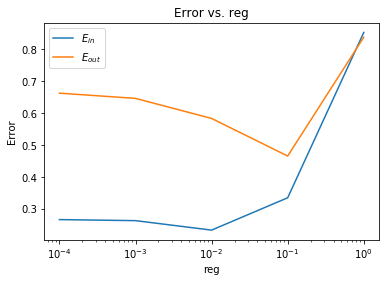
\includegraphics[width=8cm]{Pictures/2_reg}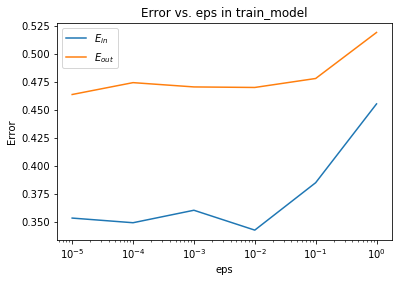
\includegraphics[width=8cm]{Pictures/2_eps}
\end{center}
Off-the-shelf implementation works by \\
*******************************************\\
TODO \\
*******************************************\\

\noindent\textbf{Differences }\\
The first two methods differ in that the first one does not have a bias while the second method does incorporate a bias. The first two methods and the off-the-shelf implementation differ by \\
*******************************************\\
TODO \\
*******************************************\\

\noindent\textbf{Performance }\\
On the test case, the normal SVD got a test error of 0.511003967792. The SVD with bias got a test error of 0.472148622408. The off-the-shelf implementation got a test error of \\
*******************************************\\
TODO \\
*******************************************\\

\noindent\textbf{Test error explanation }\\
We see that overall, the test errors were pretty high. This is due to the fact that we start of with a 943 users x 1682 movies matrix. This gives us a total of 1,586,126 values in the matrix. In the training dataset, we were only provided with 90,000 values, which means learning U and V to predict the whole matrix was a hefty task. It makes sense that our test errors were pretty high. The SVD with bias did perform better than SVD with no bias by about 4 percent. This makes sense because there is a tendency for how a user rates a movie and how a movie is rated. For example, one user may be very optimistic and give relatively high ratings for all of his/her ratings. Incorporating a bias can help us model this because then it makes sure that U and V are focused on variability between users and movies. That is, in our example, it models how that optimistic user varies between how he/she judges movies. The off-the-shelf implementation differences explain the test differences by \\
*******************************************\\
TODO \\
*******************************************\\


\newpage

\section{Matrix Factorization Visualizations [30 points]}
\noindent\textbf{General trends }\\
*******************************************\\
TODO \\
*******************************************\\
\noindent\textbf{Expectation }\\
The visuals did match what we expected to see. We expected to see some minor trends but no major trends because the test accuracies were high.  \\
\noindent\textbf{Popular vs best movies visualization }\\
We can see that in the popular movie plots, many of the movies are clustered around the origin (0, 0). These movies seem to have latent factor 1 and 2 with values close to 0. For the highest rated movies, in the plots, we can see that these movies have a more widespread distribution with varying factor 1 and 2 values. \\
*******************************************\\
TODO \\
*******************************************\\
\begin{center}
	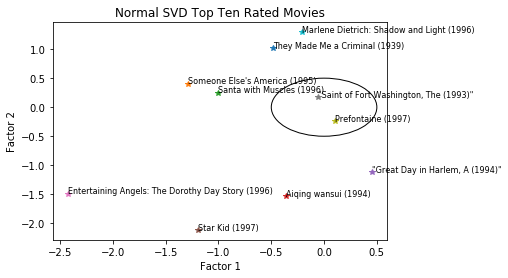
\includegraphics[width=8cm]{Pictures/1_edit1}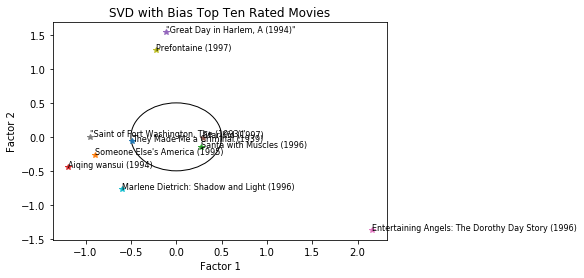
\includegraphics[width=9cm]{Pictures/2_edit1}
\end{center}
\noindent\textbf{Three genres visualization }\\
The three genres we chose were action, adventure, and animation. Looking at the plots of the combined genres, we see that in the visualization of normal SVD, the three genres were varying across the Factor 2 axis. For Factor 1, it seems like animation movies had a small factor 1 than action movies, which have a smaller factor 1 than adventure movies. Looking at the visualization for SVD with bias, we see that all three genres similarly are varying across the factor 2 axis, but in this case, adventure movies had a smaller factor 1 than action movies, which have a smaller factor 1 than animation movies. In both cases, the three genres are generally seperated vertically (we can use vertical lines to approximately seperate the three genres). \\
*******************************************\\
TODO \\
*******************************************\\
\begin{center}
	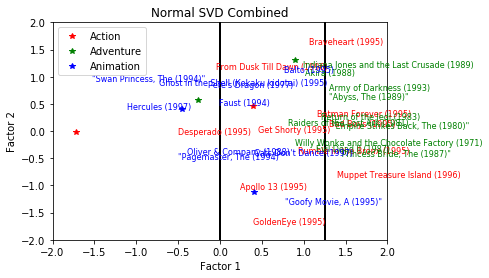
\includegraphics[width=9cm]{Pictures/1_edit}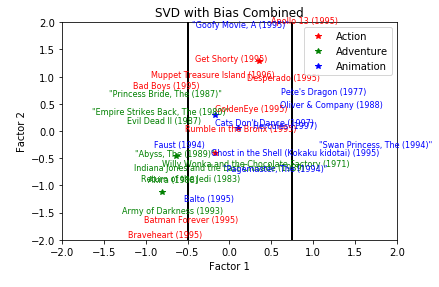
\includegraphics[width=8cm]{Pictures/2_edit}
\end{center}
\noindent\textbf{Visualization differences between methods }\\
*******************************************\\
TODO \\
*******************************************\\
\end{document}
